\section{Results}
\label{sec:results}

In order to test and compare the methods presented in \cref{sec:proposed-method},
the methods were applied to real PV time series data, described in detail in \cref{sec:data-source}.
The results shown in this section are for the PV time series covering
103 days from 21 March to 29 June, 2021.

\subsection{Day-ahead forecasts}

Using data available prior to sunrise, the proposed day-ahead forecast method from  \cref{sec:method-day-ahead} was applied to each of the weather forecast sources
(MGM meteogram cloudiness, SolCast cloudiness, and SolCast ghi)
to forecast the upcoming one-day (24 hr) PV output.
Following findings from \cite{Almeida2015},
28 days of historical data was used to fit the regression models.
In addition to the proposed method, a reference day-ahead persistence forecast was also generated.
The persistence forecast was that the PV output for the upcoming period will be the same as the PV output for the same time of day in the previous day.

Following \cite{Pedro2012} and \cite{Gigoni2018}, the methods were evaluated using mean square error (MSE), mean absolute error (MAE), and mean bias error (MBE) as the error measure.
These metrics were calculated for of the whole time series as well as the for the forecast total energy output for each day.

\begin{table}[tbh]
	\centering
	\caption{Day-ahead forecast metrics}
	\label{table:dayahead-metrics}
	\begin{tabular}{lccc}
		\toprule
		                       &   MSE    &   MAE    &    MBE    \\
        \midrule
		Persistence & 0.015722 & 0.062034 & 0.000559 \\
		%Persistence 3 Days Avg & 0.012154 & 0.056241 & 0.000765 \\
		%Persistence 28 Days Avg & 0.010510 & 0.056196 & 0.012774 \\
		SolCast Cloudiness & 0.006049 & 0.039775 & -0.008772 \\
		SolCast GHI & 0.006440 & 0.039048 & -0.011762 \\
		%MGM Meteogram1 & 0.007450 & 0.045221 & -0.007386 \\
		MGM Meteogram & 0.007343 & 0.046865 & 0.002728 \\
		\bottomrule
	\end{tabular}
\end{table}

\begin{table}[tbh]
	\centering
	\caption{Day-ahead forecast metrics on daily sums}
	\label{table:dayahead-metrics-sum}
	\begin{tabular}{lccc}
		\toprule
		                       &   MSE    &   MAE    &    MBE    \\
        \midrule
		Persistence & 2.254678 & 1.154667 & 0.013278 \\
		%Persistence 3 Days Avg & 1.849556 & 1.069204 & 0.018169 \\
		%Persistence 28 Days Avg & 1.653687 & 1.049198 & 0.303316 \\
		SolCast Cloudiness & 0.575034 & 0.583713 & -0.208281 \\
		SolCast GHI & 0.569468 & 0.564057 & -0.279288 \\
		%MGM Meteogram1 & 0.757048 & 0.676501 & -0.171603 \\
		MGM Meteogram & 0.792630 & 0.699723 & 0.063379 \\
		\bottomrule
	\end{tabular}
\end{table}

%SolCastForecasts_w_regr_out  page 41
\begin{figure}[tbh]
	\centering
	% trim=left botm right top
	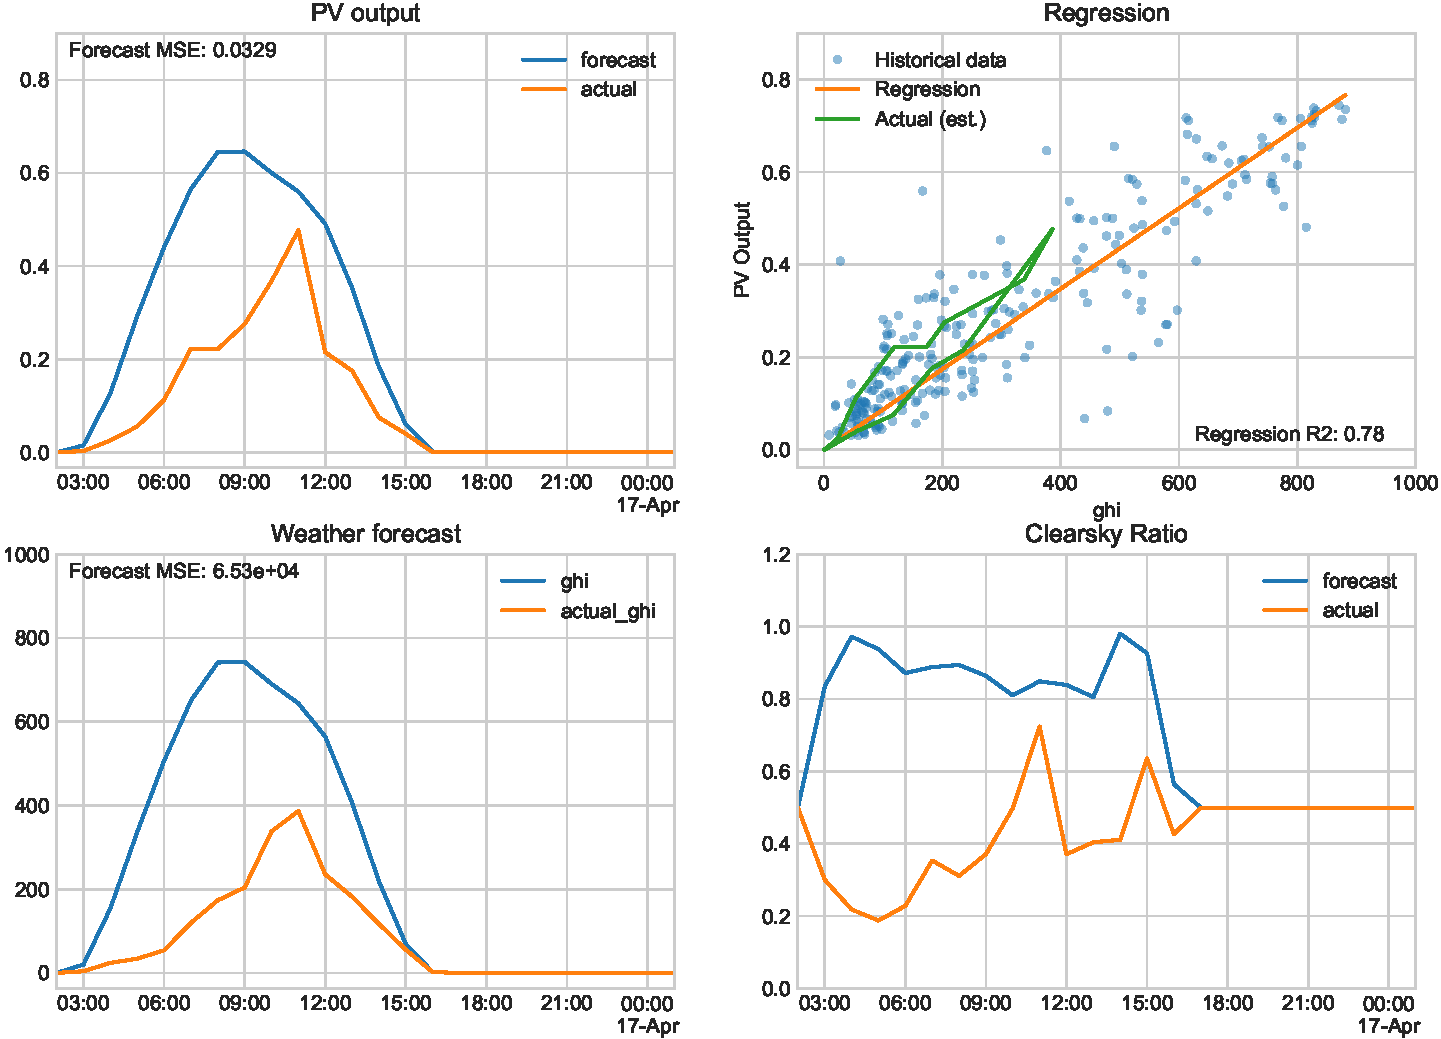
\includegraphics[width=1.0\columnwidth]{SolCastGHIForecasts-cropped.pdf}
	% Convert to png: pdftoppm SolCastForecasts_w_regr_out_p41.pdf SolCastForecasts_w_regr_out_p41 -singlefile -cropbox -png -r 1200
	%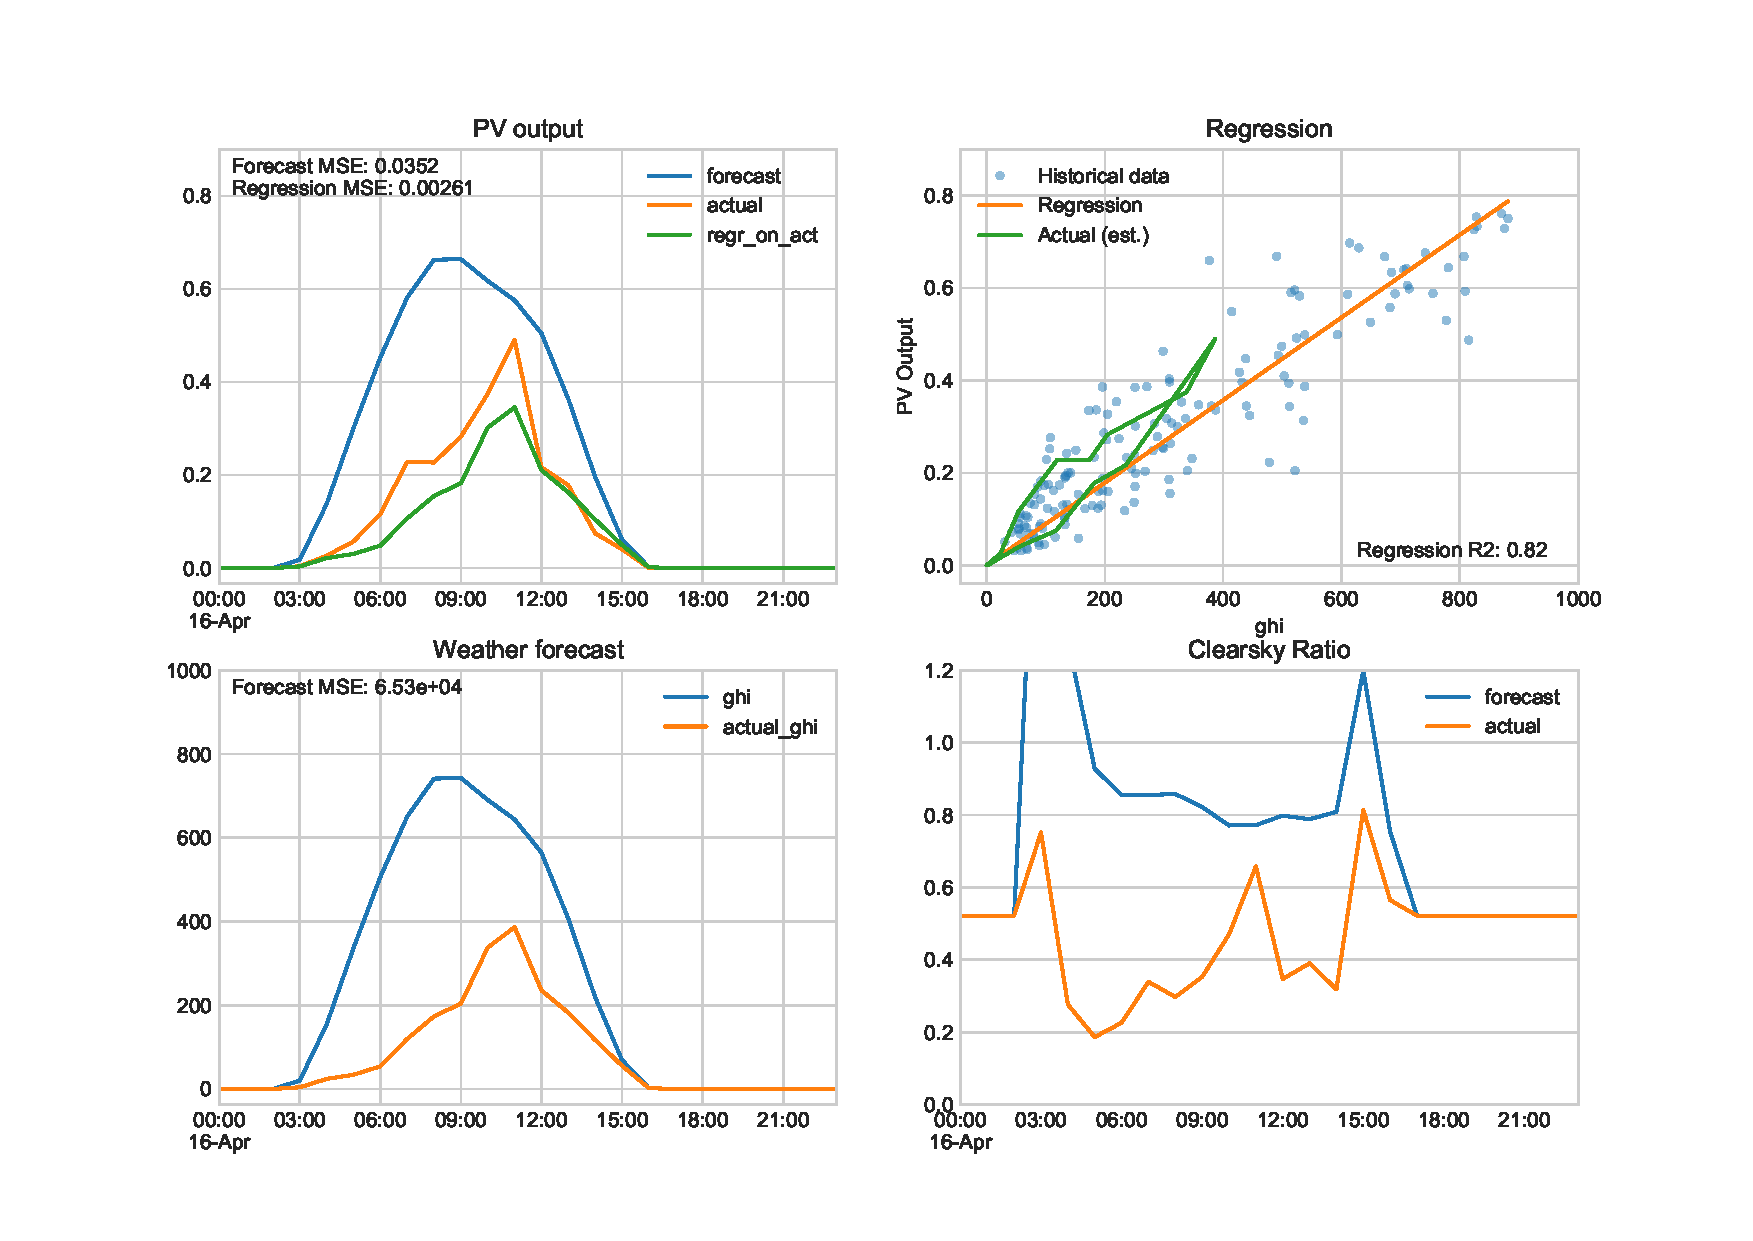
\includegraphics[width=6.5in]{SolCastForecasts_w_regr_out_p41.png}
	\caption{Example Day-ahead Forecast using Solcast GHI Forecast}
	\label{fig:dayahead-forecast-solcast}
\end{figure}


%MeteogramForecasts_cs_ratio  page 41
\begin{figure}[tbh]
	\centering
	% trim=left botm right top
	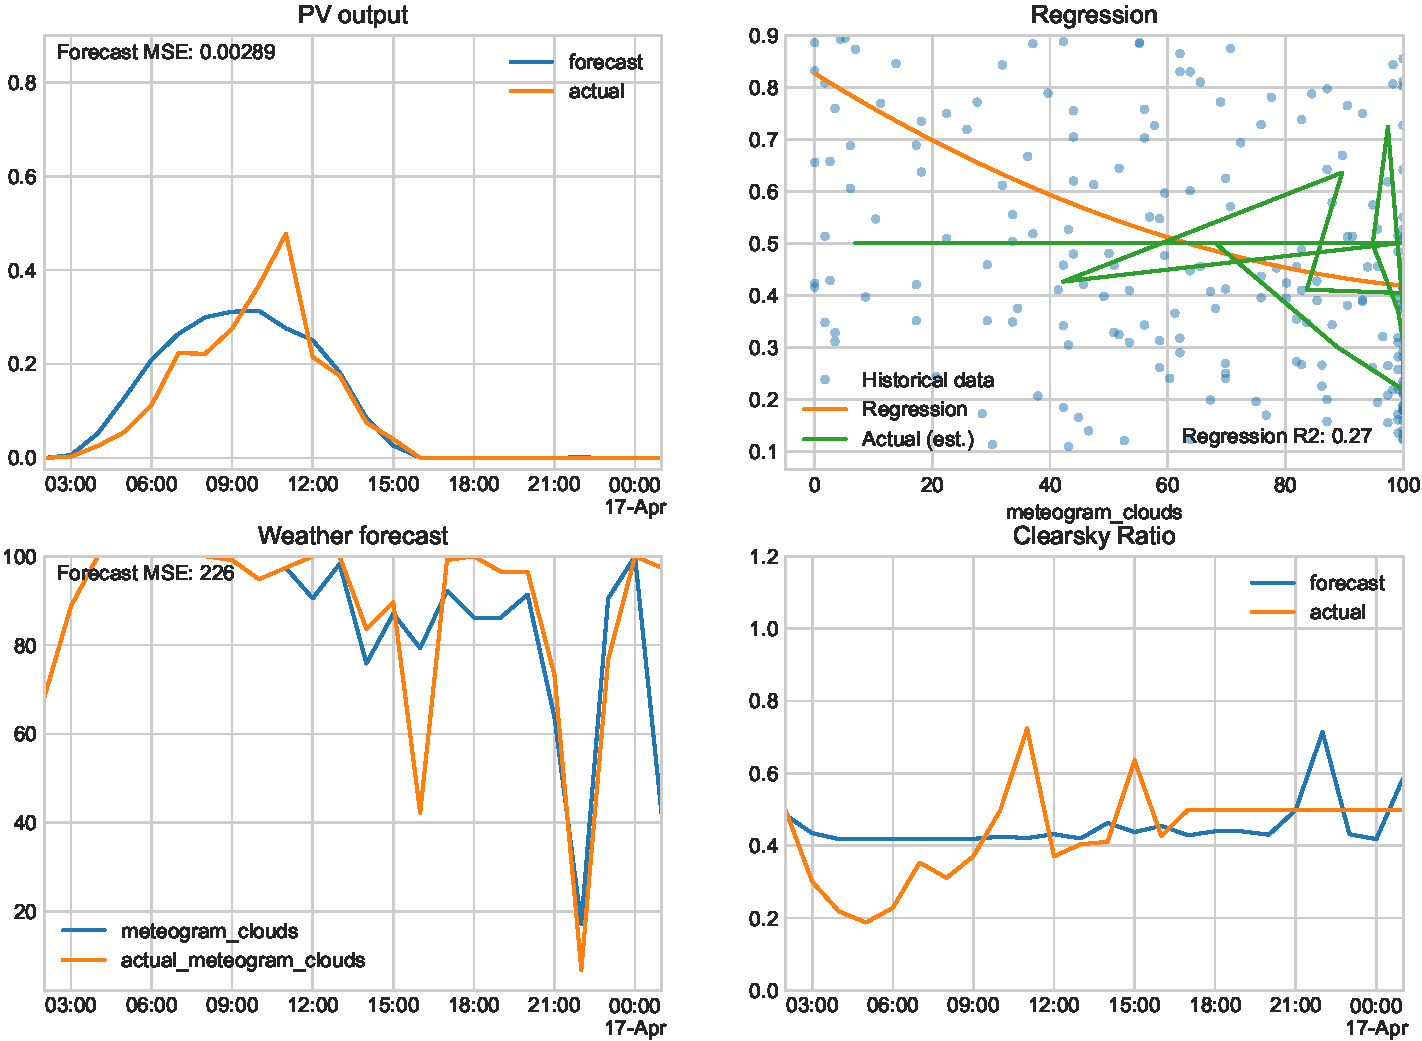
\includegraphics[width=1.0\columnwidth]{MeteogramForecasts_csratio_max-cropped.pdf}
	%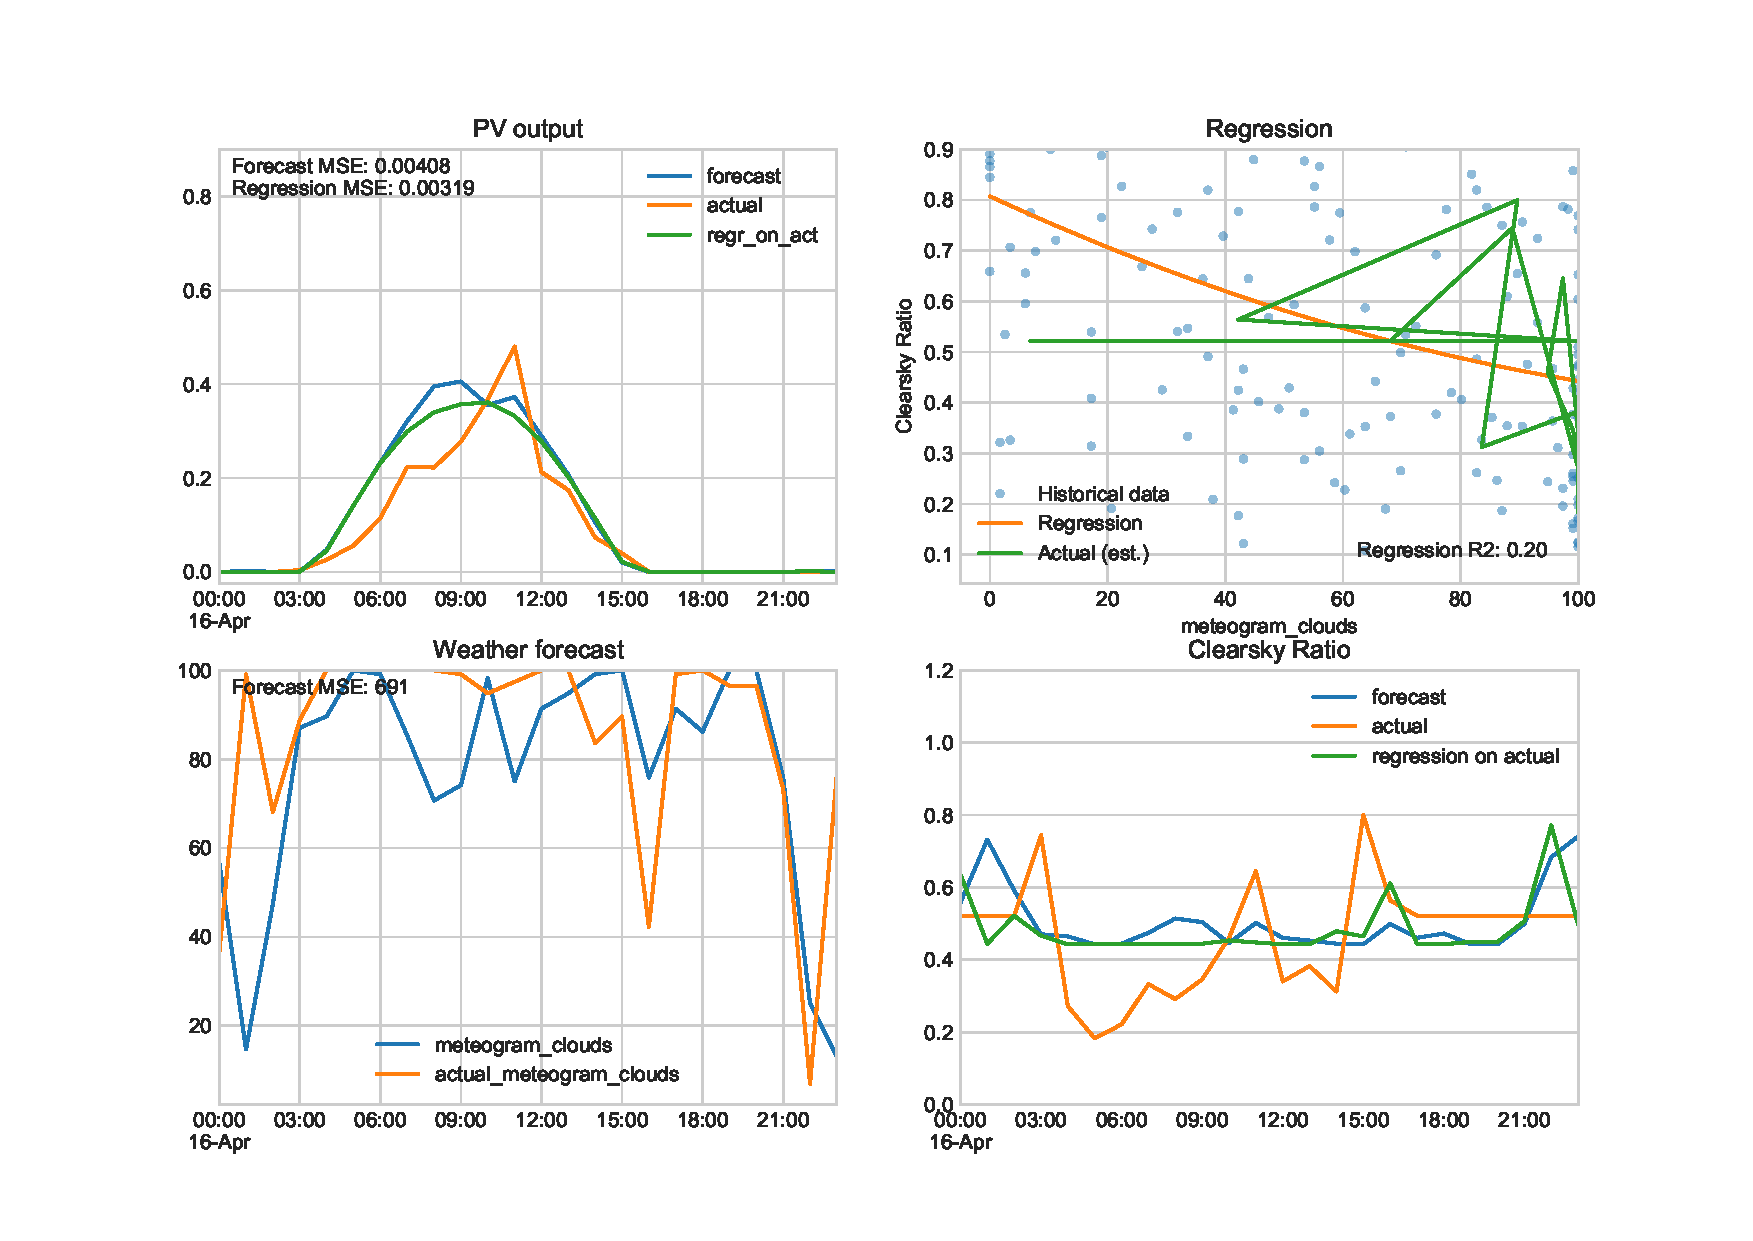
\includegraphics[width=6.5in]{MeteogramForecasts_cs_ratio_p41.png}
	\caption{Example Day-ahead Forecast using MGM Meteogram Weather Forecast}
	\label{fig:dayahead-forecast-meteogram}
\end{figure}


\subsection{Intra-day Updates}

To evaluate and compare the intra-day forecast update methods,
as a starting point, a day-ahead forecast was first generated using the
SolCast cloudiness forecast.
This day-ahead forecast was then updated for each hour of the day using each of the methods proposed in \cref{sec:method-intraday}.
In addition to the proposed methods, a reference intra-day update forecast based on persistence was produced.
The persistence forecast was that the clear-sky ratio for the remainder of the day would be the same as the clear-sky ratio from the previous time period.

For comparison, the MSE for the different intra-day forecast update methods was computed for the forecast for one hour, two hours, and six hours ahead. The result error metrics are shown in \cref{table:intraday-metrics}.

\begin{table}
	\centering
\begin{threeparttable}
	\caption{Intraday forecast metrics}
	\label{table:intraday-metrics}
	\begin{tabular}{clccc}
		\toprule
		\shortstack{Hours\\Ahead} & Method & MSE & MAE & MBE \\
		\midrule
		%A & B & C\tnote{1} & D & E\tnote{1} \\
		%G & H\tnote{2} & I & J & K \\
		\multirow[c]{6}{*}{1} & Persistence & 0.004409 & 0.032320 & -0.001955 \\
		& fx\_output\tnote{1} & 0.003743 & 0.031664 & -0.003686 \\
		& fx\_csratio\tnote{2} & 0.003803 & 0.033566 & 0.006633 \\
		& exog\tnote{3} & 0.003917 & 0.035667 & 0.008020 \\
		& SARIMAX & 0.003726 & 0.032159 & -0.001687 \\
		& Scaling & 0.004425 & 0.032737 & 0.000284 \\
		\midrule
		\multirow[c]{6}{*}{2} & Persistence & 0.007663 & 0.041868 & -0.002397 \\
		& fx\_output\tnote{1} & 0.005233 & 0.037428 & -0.005418 \\
		& fx\_csratio\tnote{2} & 0.005684 & 0.041822 & 0.011613 \\
		& exog\tnote{3} & 0.006098 & 0.045131 & 0.013845 \\
		& SARIMAX & 0.005166 & 0.037879 & -0.002296 \\
		& Scaling & 0.007671 & 0.042636 & 0.001627 \\
		\midrule
		\multirow[c]{6}{*}{6} & persistence & 0.009497 & 0.047607 & -0.007485 \\
		& fx\_output\tnote{1} & 0.005756 & 0.039047 & -0.007912 \\
		& fx\_csratio\tnote{2} & 0.006253 & 0.042456 & 0.003602 \\
		& exog\tnote{3} & 0.006594 & 0.044206 & 0.003111 \\
		& SARIMAX & 0.005675 & 0.038983 & -0.006740 \\
		& Scaling & 0.009314 & 0.046933 & -0.000351 \\
		\bottomrule
	\end{tabular}
	\begin{tablenotes}
		\footnotesize
		\item[1] AR(2) on residual of PV output.
		\item[2] AR(2) on residual of clear-sky ratio
		\item[3] AR(2) on actual output with exogenous variable
	\end{tablenotes}
\end{threeparttable}
\end{table}


%\begin{table}[tbh]
%	%\centering
%	\begin{threeparttable}[b]
%	\caption{Intraday forecast metrics}
%	\label{table:intraday-metrics}
%\begin{tabular}{clccc}
%	\toprule
%	\shortstack{Hours\\Ahead} & Method & MSE & MAE & MBE \\
%	\midrule
%	\multirow[c]{6}{*}{1} & Persistence & 0.004409 & 0.032320 & -0.001955 \\
%	& fx\_output\tnote{1} & 0.003743 & 0.031664 & -0.003686 \\
%	& fx\_csratio\tnote{2} & 0.003803 & 0.033566 & 0.006633 \\
%	& exog\tnote{3} & 0.003917 & 0.035667 & 0.008020 \\
%	& sarimax & 0.003726 & 0.032159 & -0.001687 \\
%	& scaling & 0.004425 & 0.032737 & 0.000284 \\
%	\midrule
%	\multirow[c]{6}{*}{2} & Persistence & 0.007663 & 0.041868 & -0.002397 \\
%	& fx\_output\tnote{1} & 0.005233 & 0.037428 & -0.005418 \\
%	& fx\_csratio\tnote{2} & 0.005684 & 0.041822 & 0.011613 \\
%	& exog\tnote{3} & 0.006098 & 0.045131 & 0.013845 \\
%	& SARIMAX & 0.005166 & 0.037879 & -0.002296 \\
%	& Scaling & 0.007671 & 0.042636 & 0.001627 \\
%	\midrule
%%	\multirow[c]{6}{*}{2} & persistence & 0.008979 & 0.045546 & -0.003484 \\
%%	& fx\_output & 0.005466 & 0.038242 & -0.006428 \\
%%	& fx\_csratio & 0.006135 & 0.044152 & 0.013051 \\
%%	& exog & 0.006836 & 0.048039 & 0.015323 \\
%%	& sarimax & 0.005388 & 0.038507 & -0.002922 \\
%%	& scaling & 0.008988 & 0.046789 & 0.002116 \\
%%	\midrule
%	\multirow[c]{6}{*}{6} & persistence & 0.009497 & 0.047607 & -0.007485 \\
%	& fx\_output\tnote{1} & 0.005756 & 0.039047 & -0.007912 \\
%	& fx\_csratio\tnote{2} & 0.006253 & 0.042456 & 0.003602 \\
%	& exog\tnote{3} & 0.006594 & 0.044206 & 0.003111 \\
%	& SARIMAX & 0.005675 & 0.038983 & -0.006740 \\
%	& Scaling & 0.009314 & 0.046933 & -0.000351 \\
%	\bottomrule
%	\begin{tablenotes}
%		\footnotesize
%		\item[1] AR(2) on residual of PV output.
%		\item[2] AR(2) on residual of clear-sky ratio
%		\item[3] AR(2) on actual output with exogenous variable
%	\end{tablenotes}
%\end{threeparttable}
%\end{tabular}
%
%\end{table}

\begin{figure}[tbh]
	\centering
	% trim=left botm right top
	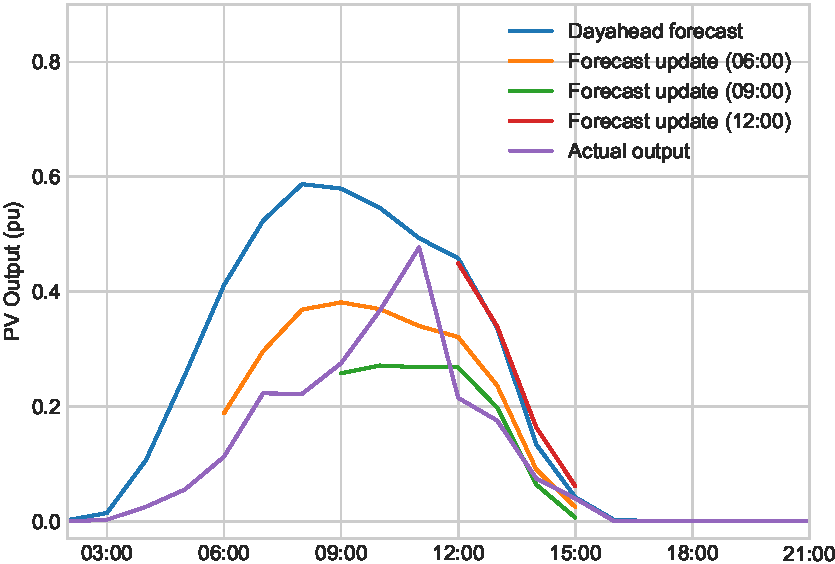
\includegraphics[width=0.85\columnwidth]{IntradayUpdate-sarimax-cropped.pdf}
	%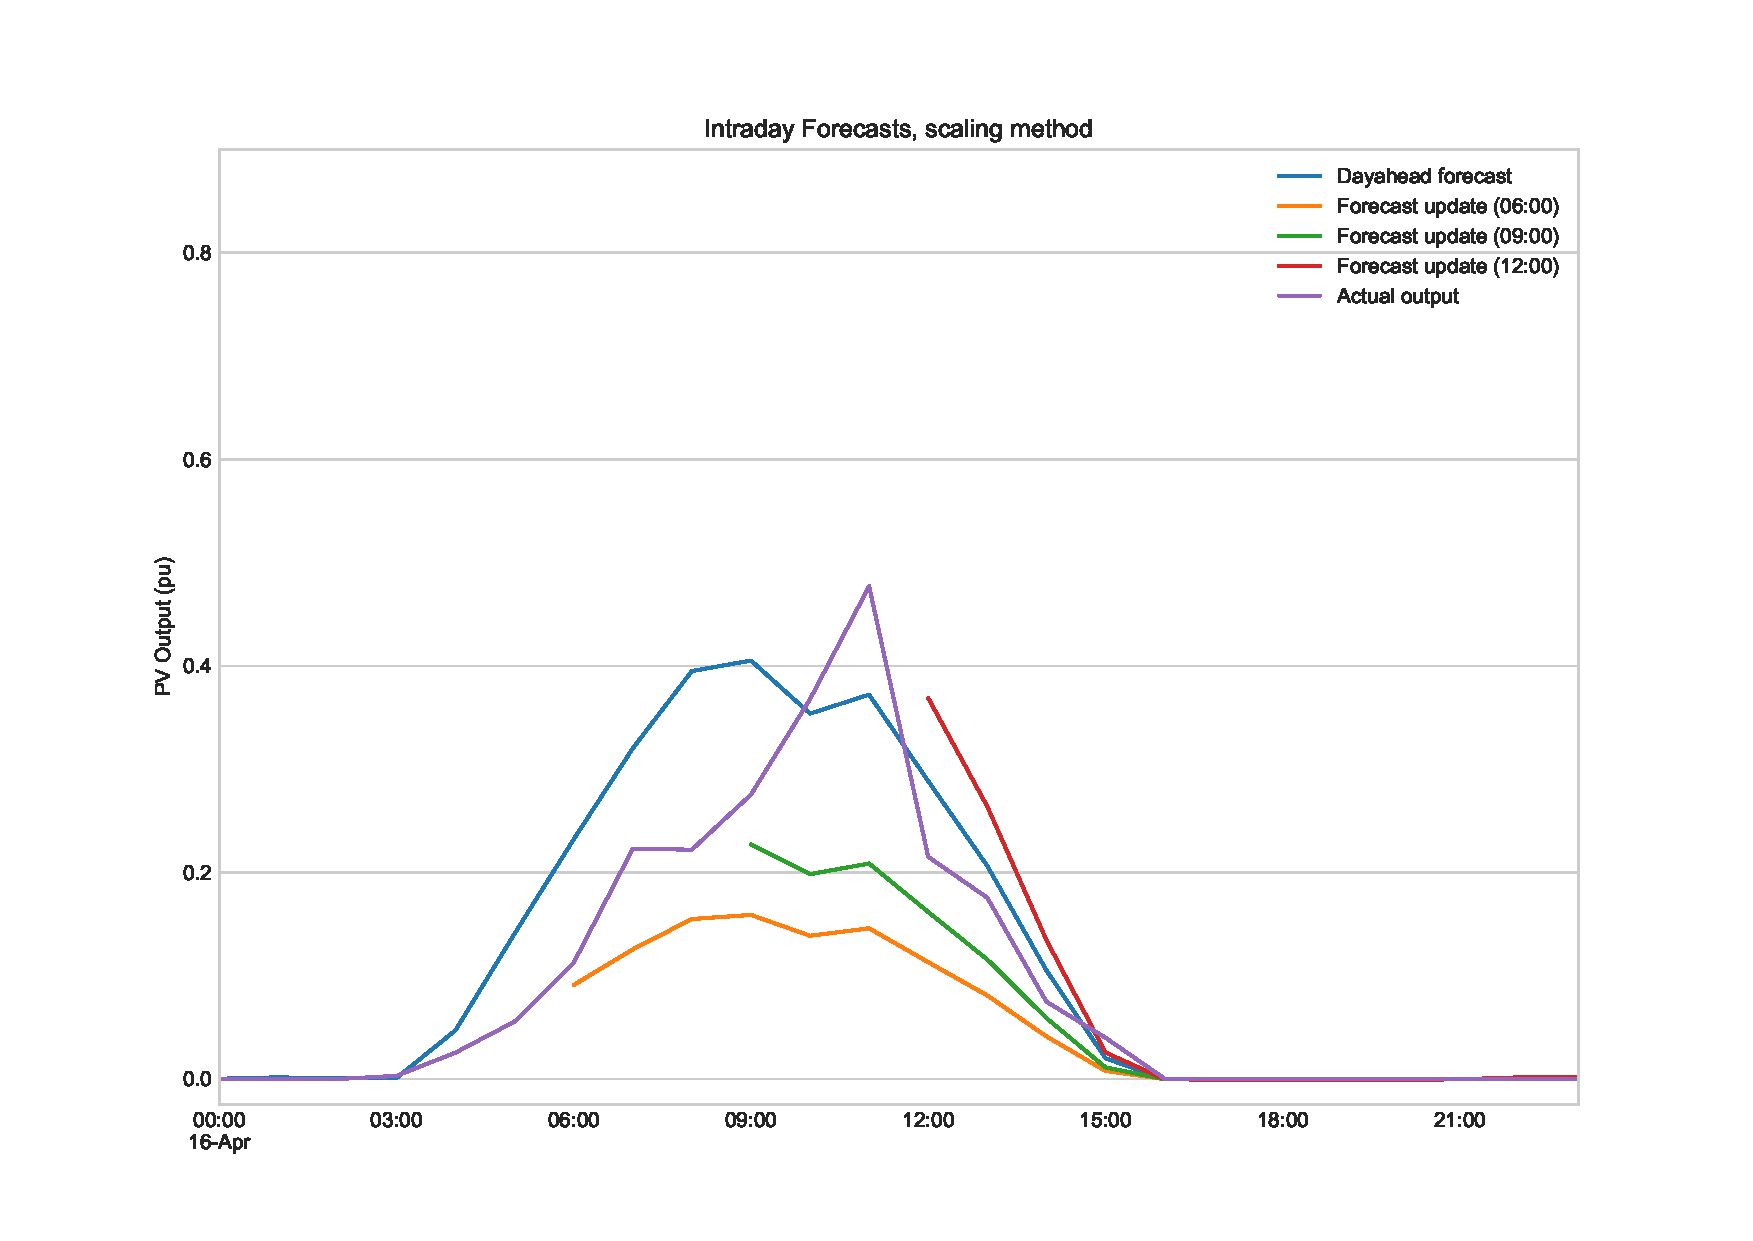
\includegraphics[width=5.53in]{Intraday Forecasts_p4.png}
	\caption{Intra-day Forecast Updates - SARIMAX method}
	\label{fig:intraday-forecast}
\end{figure}


\subsection{Optimal Energy Dispatch}

To demonstrate the effectiveness of the developed methods in the target application,
the forecasts were input into an agricultural microgrid operational optimization and simulation program.
A system diagram of the demonstration system is shown in \cref{fig:demo-system}.
The optimization formulation was previously presented in \cite{Brown2022}.
The use of model-predictive control (MPC) was simulated by using the optimizer to choose the optimal ratio of using excess available PV energy between energy storage in a battery energy storage system (BSS) and utilization to pump water into a reservoir.
The MPC optimization was performed using the forecast PV data, including intra-day updates.
The operation for the following period was then simulated using actual PV data.
A flowchart of the MPC simulation is shown in \cref{fig:mpc-simulation-flowchart}.

\begin{figure}[t]
	\centering
	\fontsize{6.7pt}{9pt}\selectfont
	\def\svgwidth{0.8\columnwidth}
	\input{figs/demo_system.pdf_tex}
	\caption{Energy Dispatch Demonstration System}
	\label{fig:demo-system}
\end{figure}

% Figure copied from last progress report
\begin{figure}[tbh]
	\centering
	% trim=left botm right top
	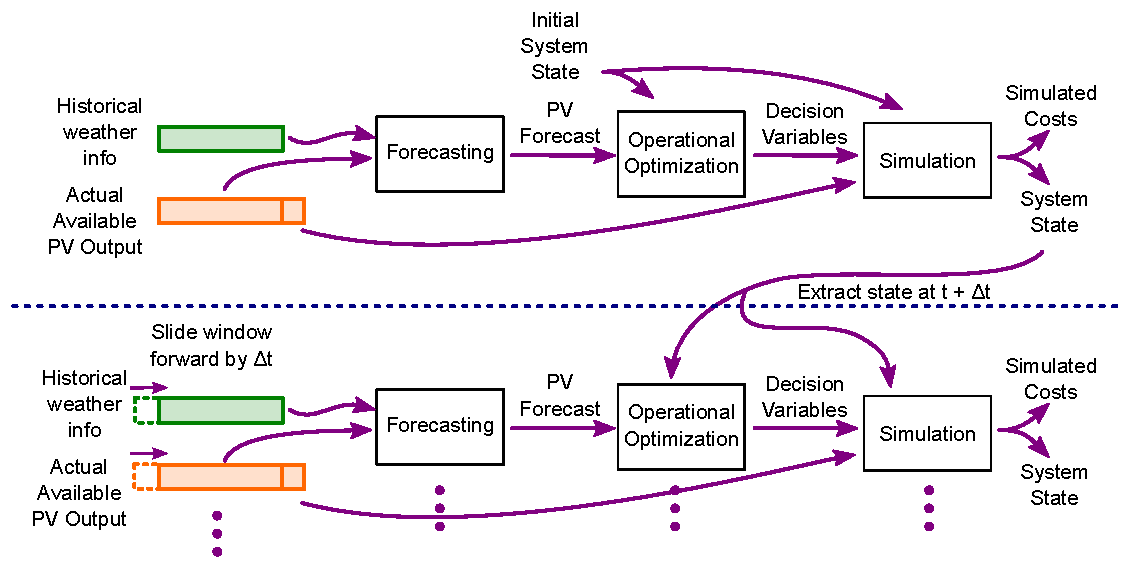
\includegraphics[width=1.0\columnwidth]{MPC Demo System Diagram.pdf}
	\caption{MPC demonstration simulation flowchart}
	\label{fig:mpc-simulation-flowchart}
\end{figure}

\Cref{table:mpc-simulation-results} shows results of the MPC simulation. Simulations were performed for three forecasts:
\begin{itemize}
\item Persistence forecast
\item SolCast cloudiness weather forecasts for day-ahead forecast with SARIMAX-based intraday updates
\item Perfect ``oracle'' forecast where operation is optimized with the actual future PV output data
\end{itemize}
The costs for the system's simulated operation using persistence forecasts were somewhat better than the performance using the proposed method.
This may potentially be explained by the relatively better bias error performance of the persistence forecasts.
Additional investigation to further improve the forecasting method may be warranted.

The objective function value for optimized operation with a perfect forecast illustrates the value of improved forecasts.

\begin{table}
	\caption{MPC Simulation Results - Objective Function Value}
	\label{table:mpc-simulation-results}
	\centering
	\begin{tabular}{lS[table-format=5]S[table-format=5]S[table-format=5]}
		\toprule
          & {\shortstack{Persistence\\Forecast}} & {\shortstack{Proposed\\Method}} & {\shortstack{Perfect\\Forecast}} \\
		  & {(\$, 2020)} & {(\$, 2020)}                    & {(\$, 2020)} \\
		\midrule
		Grid energy cost            & 65350 & 72195 & 58052 \\
		Battery use cost            &  8120 &  7979 &  8047 \\
		Inadequate water cost       &    90 &    99 &     0 \\
		Battery mode switching cost &   246 &   244 &   230 \\
		Pump switching cost         &    94 &   104 &    80 \\
		\midrule
		TOTAL                       & 82846 & 90474 & 66418 \\
		\bottomrule
	\end{tabular}
\end{table}

